\documentclass[journal,12pt,twocolumn]{IEEEtran}

\usepackage{setspace}
\usepackage{gensymb}
\singlespacing
\usepackage[cmex10]{amsmath}
\usepackage{amssymb}
\usepackage{xurl}
\usepackage{tabularx}
\usepackage{amsthm}
\usepackage{comment}
\usepackage{mathrsfs}
\usepackage{txfonts}
\usepackage{stfloats}
\usepackage{bm}
\usepackage{cite}
\usepackage{cases}
\usepackage{subfig}

\usepackage{longtable}
\usepackage{multirow}

\usepackage{enumitem}
\usepackage{mathtools}
\usepackage{steinmetz}
\usepackage{tikz}
\usepackage{circuitikz}
\usepackage{verbatim}
\usepackage{tfrupee}
\usepackage[breaklinks=true]{hyperref}
\usepackage{graphicx}
\usepackage{tkz-euclide}

\usetikzlibrary{calc,math}
\usepackage{listings}
    \usepackage{color}                                            %%
    \usepackage{array}                                            %%
    \usepackage{longtable}                                        %%
    \usepackage{calc}                                             %%
    \usepackage{multirow}                                         %%
    \usepackage{hhline}                                           %%
    \usepackage{ifthen}                                           %%
    \usepackage{lscape}     
\usepackage{multicol}
\usepackage{chngcntr}

\DeclareMathOperator*{\Res}{Res}

\renewcommand\thesection{\arabic{section}}
\renewcommand\thesubsection{\thesection.\arabic{subsection}}
\renewcommand\thesubsubsection{\thesubsection.\arabic{subsubsection}}

\renewcommand\thesectiondis{\arabic{section}}
\renewcommand\thesubsectiondis{\thesectiondis.\arabic{subsection}}
\renewcommand\thesubsubsectiondis{\thesubsectiondis.\arabic{subsubsection}}


\hyphenation{op-tical net-works semi-conduc-tor}
\def\inputGnumericTable{}                                 %%

\lstset{
%language=C,
frame=single, 
breaklines=true,
columns=fullflexible
}
\begin{document}


\newtheorem{theorem}{Theorem}[section]
\newtheorem{problem}{Problem}
\newtheorem{proposition}{Proposition}[section]
\newtheorem{lemma}{Lemma}[section]
\newtheorem{corollary}[theorem]{Corollary}
\newtheorem{example}{Example}[section]
\newtheorem{definition}[problem]{Definition}

\newcommand{\BEQA}{\begin{eqnarray}}
\newcommand{\EEQA}{\end{eqnarray}}
\newcommand{\define}{\stackrel{\triangle}{=}}
\bibliographystyle{IEEEtran}
\raggedbottom
\setlength{\parindent}{0pt}
\providecommand{\mbf}{\mathbf}
\providecommand{\pr}[1]{\ensuremath{\Pr\left(#1\right)}}
\providecommand{\qfunc}[1]{\ensuremath{Q\left(#1\right)}}
\providecommand{\sbrak}[1]{\ensuremath{{}\left[#1\right]}}
\providecommand{\lsbrak}[1]{\ensuremath{{}\left[#1\right.}}
\providecommand{\rsbrak}[1]{\ensuremath{{}\left.#1\right]}}
\providecommand{\brak}[1]{\ensuremath{\left(#1\right)}}
\providecommand{\lbrak}[1]{\ensuremath{\left(#1\right.}}
\providecommand{\rbrak}[1]{\ensuremath{\left.#1\right)}}
\providecommand{\cbrak}[1]{\ensuremath{\left\{#1\right\}}}
\providecommand{\lcbrak}[1]{\ensuremath{\left\{#1\right.}}
\providecommand{\rcbrak}[1]{\ensuremath{\left.#1\right\}}}
\theoremstyle{remark}
\newtheorem{rem}{Remark}
\newcommand{\sgn}{\mathop{\mathrm{sgn}}}
\providecommand{\abs}[1]{\vert#1\vert}
\providecommand{\res}[1]{\Res\displaylimits_{#1}} 
\providecommand{\norm}[1]{\lVert#1\rVert}
%\providecommand{\norm}[1]{\lVert#1\rVert}
\providecommand{\mtx}[1]{\mathbf{#1}}
\providecommand{\mean}[1]{E[ #1 ]}
\providecommand{\fourier}{\overset{\mathcal{F}}{ \rightleftharpoons}}
%\providecommand{\hilbert}{\overset{\mathcal{H}}{ \rightleftharpoons}}
\providecommand{\system}{\overset{\mathcal{H}}{ \longleftrightarrow}}
	%\newcommand{\solution}[2]{\textbf{Solution:}{#1}}
\newcommand{\solution}{\noindent \textbf{Solution: }}
\newcommand{\cosec}{\,\text{cosec}\,}
\providecommand{\dec}[2]{\ensuremath{\overset{#1}{\underset{#2}{\gtrless}}}}
\newcommand{\myvec}[1]{\ensuremath{\begin{pmatrix}#1\end{pmatrix}}}
\newcommand{\mydet}[1]{\ensuremath{\begin{vmatrix}#1\end{vmatrix}}}
\newcommand*{\permcomb}[4][0mu]{{{}^{#3}\mkern#1#2_{#4}}}
\newcommand*{\perm}[1][-3mu]{\permcomb[#1]{P}}
\newcommand*{\comb}[1][-1mu]{\permcomb[#1]{C}}
\numberwithin{equation}{subsection}
\makeatletter
\@addtoreset{figure}{problem}
\makeatother
\let\StandardTheFigure\thefigure
\let\vec\mathbf
\renewcommand{\thefigure}{\theproblem}
\def\putbox#1#2#3{\makebox[0in][l]{\makebox[#1][l]{}\raisebox{\baselineskip}[0in][0in]{\raisebox{#2}[0in][0in]{#3}}}}
     \def\rightbox#1{\makebox[0in][r]{#1}}
     \def\centbox#1{\makebox[0in]{#1}}
     \def\topbox#1{\raisebox{-\baselineskip}[0in][0in]{#1}}
     \def\midbox#1{\raisebox{-0.5\baselineskip}[0in][0in]{#1}}
\vspace{3cm}
\title{AI1103 : Assignment 3}
\author{Yashas Tadikamalla - AI20BTECH11027}
\maketitle
\newpage
\bigskip
\renewcommand{\thefigure}{\arabic{figure}}
\renewcommand{\thetable}{\arabic{table}}
Download all python codes from 
\begin{lstlisting}
https://github.com/YashasTadikamalla/AI1103/tree/main/Assignment3/codes
\end{lstlisting}
%
and latex codes from 
%
\begin{lstlisting}
https://github.com/YashasTadikamalla/AI1103/blob/main/Assignment3/Assignment3.tex
\end{lstlisting}
\section*{Problem(GATE-26)}

A fair dice is tossed two times. The probability that the second toss result in a value that is higher than the first toss is
\newline
\newline
(A)$\dfrac{2}{36}\hspace{0.5cm}$ (B)$\dfrac{2}{6}\hspace{0.5cm}$  (C)$\dfrac{5}{12}\hspace{0.5cm}$  (D)$\dfrac{1}{2}\hspace{0.5cm}$
\section*{Solution(GATE-26)}

Given, a fair die, which is tossed twice. Let the random variable $X_{i}\in\{1,2,3,4,5,6\},i=1,2,$ represent the outcome of the number on the die in the first, second toss. $X_{1},X_{2}$ denote the result of the first, second toss respectively.
\newline
\newline
As the die is given to be fair, the probability  mass function (PMF) is expressed as \begin{align}
    \tag{26.1}
    p_{X_{i}}(n)=\Pr(X_{i}=n) = 
	\begin{cases}
	\dfrac{1}{6}, & 1\leq n\leq6 \\~\\[-1em]
	0, & otherwise
	\end{cases}
	\label{eq:pmf}
\end{align}
\newline
The desired outcome $X_{1}<X_{2}$, is of the form
\begin{align}
    \tag{26.2}
    X_{1}\leq n-1,X_{2}=n
\end{align}
The probability for this outcome is of the form
\begin{multline}
    \tag{26.3}
    Pr(X_{1}\leq n-1,X_{2}=n)\\=Pr(X_{2}=n) \times Pr(X_{1}\leq n-1/X_{2}=n)
    \label{eq:probeqn}
\end{multline}
As $X_{1},X_{2}$ are independent, \eqref{eq:probeqn} simplifies to
\begin{multline}
    \tag{26.4}
    \label{eq:exprsn}
    Pr(X_{1}\leq n-1,X_{2}=n)\\=Pr(X_{2}=n) \times Pr(X_{1}\leq n-1)
\end{multline}
\eqref{eq:exprsn} can be rewritten as
\begin{multline}
    \tag{26.5}
    Pr(X_{1}\leq n-1,X_{2}=n)\\=p_{X_{2}}(n) \times F_{X_{1}}(n-1)
\end{multline}
Using \eqref{eq:pmf}, the cumulative distribution function (CDF) is obtained to be
\begin{align}
    \tag{26.6}
    F_{X_{i}}(r)=\Pr(X_{i}\leq n) = 
	\begin{cases}
	\dfrac{n}{6}, & 1\leq n\leq6 \\~\\[-1em]
	1, & n \geq 7 \\~\\[-1em]
	0, & otherwise
	\end{cases}
	\label{eq:26.6}
\end{align}
\newline
Hence the required probability is
\begin{multline}
    \tag{26.7}
    \sum_{n=1}^{n=6}Pr(X_{1}\leq n-1,X_{2}=n)\\=\sum_{n=1}^{n=6}p_{X_{2}}(n) \times F_{X_{1}}(n-1)
\end{multline}
From \eqref{eq:pmf} and \eqref{eq:26.6},
\begin{align}
    \tag{26.8}
    \sum_{n=1}^{n=6}Pr(X_{1}\leq n-1,X_{2}=n)=\sum_{n=1}^{n=6}\dfrac{1}{6}\times\dfrac{n-1}{6} 
    \label{eq:finalexpsn}
\end{align}
On solving \eqref{eq:finalexpsn}, we get
\begin{align}
    \tag{26.9}
    \sum_{n=1}^{n=6}Pr(X_{1}\leq n-1,X_{2}=n)=\dfrac{5}{12} \\
    \tag{26.10}
    \therefore Pr(X_{1}<X_{2})=\dfrac{5}{12}\text{(option (C))}
\end{align}
P.T.O
\newpage
\begin{table}[h!]
\centering
\caption{Theoretical probabilities for different possible cases}
\label{table:1}
\begin{tabular}{|c||c|c|c|}
    \hline
    Condition & $X_{1}<X_{2}$& $X_{1}>X_{2}$& $X_{1}=X_{2}$ \\
    \hline
    %& & &\\
    Probability & $\dfrac{5}{12}$ & $\dfrac{5}{12}$ & $\dfrac{1}{12}$\\[1ex]
    \hline
\end{tabular}
\end{table}
Here is the plot describing the Theoretical vs Simulation results for the above mentioned cases
\newline
\newline
\centering
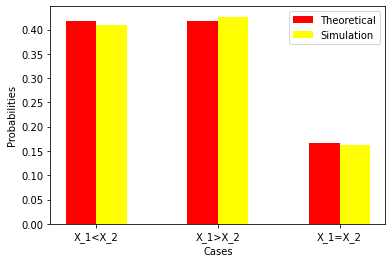
\includegraphics[scale=0.6]{Assignment3.png}
\end{document}